\chapter{Retail Site Decision Process}
\label{ch:2}

The retail sector is currently in a phase of transformation due to various factors, including the rise in consumer mobility, the prevalence of e-commerce, shifting household demographics, and market saturation. With that, there were evolving 
business strategies to align with emerging trends. Since the late 1970s, there has been a noticeable decline in the growth of hypermarkets, with small and medium-sized supermarkets gaining preference. This shift in consumer behaviour has forced small retailers to adopt more strategic approaches when selecting store locations, determining store size, and offering services \cite{mendes2004multi}.

This section aims to conduct a concise analysis of the algorithms and methodologies mentioned in research \cite{roig2013retail}. It aims to examine their strengths and weaknesses and explore alternative options available on a global scale. The section is structured so that each subsection explains a specific step within the research (Figure \ref{fig:system-diagram}).

The methodology implies two critical concepts based on spatial dispersion: \textit{Geo-demand} and \textit{Geo-competition}. Geo-demand is the location of potential customers. Geo-competition is the location of business competitors \cite{baviera2012trade}. Each concept is going to contain data points that can be outlined on a map within separate layers. First layer will contain density of the customers on a map, the second layer should contain estimated trading areas of the competitors \cite{roig2013retail}. Once these two layers are identified, the third layer can be obtained by their joint analysis \cite{baviera2012trade}. The third layer should reveal areas where commercial service is poor, and population density is high. These areas are then considered good for outlets---at this point, a retailer can determine potential sites for his business. 

In the next step decision-maker must provide attributes for each potential location, which he can then compare against each other using 1-9 scales, for instance, attribute $A$ is 9 times more important for him than attribute $B$. 

Once it is done, \textit{Analytic Hierarchy Process} (AHP) is applied in order to evaluate all the attributes on each site and output locations with their rating. The location that contains the greatest value of the rating is considered to be the most desired. The consistency of the output fully depends on the user \cite{roig2013retail}.

\newpage

\begin{figure}[ht]
	\centering
	\includesvg[width=0.6\textwidth]{obrazky-figures/ch2/system-diagram.svg}
	\caption{Process flow diagram (Adapted from \cite{roig2013retail})}
	\label{fig:system-diagram}
\end{figure}

\section{Identifying Geo-demand}

Geo-demand can be defined as the location of potential customers who purchase a product or service in a specific market (Figure~\ref{fig:geo-demand}). According to \cite{roig2013retail}, individuals who live in the area can be viewed as potential customers. This is due to the possibility that individuals might express interest in various markets without certainty regarding their preferences. The data for geo-demand can be acquired from the local city database.

\begin{figure}[ht]
	\centering
	\includesvg[width=1\textwidth]{obrazky-figures/ch2/geo-demand.svg}
	\caption{Example of geo-demand in Brno. Each blue point represents the location of potential customers.}
	\label{fig:geo-demand}
\end{figure}

\section{Identifying Geo-competition}
\label{sec:identifyingGeocompetition}

Geo-competition is the location of the competitors of a business and the delineation of their trade areas in a particular market. Trade area can be defined as the geographic area in which a retailer attracts customers \cite{baviera2012trade, roig2013retail}.

Geo-competition is more complicated than the previous step \cite{roig2013retail}. In the last decade, people have created tons of procedures and algorithms that can help to identify trading areas. The procedure for this thesis targets theoretical method, specifically the probabilistic model invented by David L. Huff in 1964 to identify geo-competition, but for completeness of analysis, this section will briefly describe the development of theoretical methods to understand their strengths, weaknesses and challenges \cite{roig2013retail}.

\subsection{Development of Theoretical Methods}

Theoretical methods for defining trading areas involve developing conceptual frameworks or models that explain the spatial interactions and patterns associated with trade or business activities. These methods are based on theoretical principles about how certain factors influence the formation of trading areas \cite{mendes2004multi}.

\begin{itemize}
    \item \textbf{Gravity Models}---theoretical frameworks borrowed from physics. They are derived from the laws of Newtonian physics, based on the balance between the store attractivity and the distance to the potential customers \cite{mendes2004multi}.
    \item \textbf{Probabilistic Models}---models that are based on the likelihood of customers visiting a certain location within a specific geographical region \cite{huff1964defining}.
\end{itemize}

\subsubsection{J. Reilly's Model}

One of the first studies that developed theoretical methods was done by William J. Reilly who formalized a number of empirical observations concerning consumer shopping movements between cities \cite{huff1964defining}.

 The idea is that people prefer shopping in bigger communities, but the distance and time it takes to get there affect their willingness to do so in a particular city. In simpler terms, people tend to choose shorter travel distances when they can. Moreover, larger communities are more appealing to shoppers because they usually have a greater variety of products and services (Figure \ref{fig:reilyModel}) \cite{web2022trade}.

\begin{figure}[t]
	\centering
	\includesvg[width=1\textwidth]{obrazky-figures/ch2/reilly-model.svg}
	\caption{This is a map of Waupaca, Wisconsin, USA. The map shows the location of a town, Waupaca, along with surrounding communities. Based on community populations and their distribution, it is possible to draw a simple trade area using the concepts of Reilly’s Law (Adopted from \cite{tradeareaanalysis})}
\label{fig:reilyModel}
\end{figure}

The retail gravitation model has the following structure:
\begin{equation}
\frac{B_a}{B_b}= \left( \frac{P_a}{P_b} \right) \left( \frac{D_b}{D_a} \right)^2
\label{WilliamEquation}
\end{equation}

\begin{itemize}
    \item{$B_a$ = the proportion of the retail business from an intermediate town attracted by city $A$ (Size or buying power of City A's trade area)}
    \item{$B_b$ = the proportion of the retail business from an intermediate town attracted by city $B$ (Size or buying power of City B's trade area)}
    \item{$P_a$ = the population of city $A$}
    \item{$P_b$ = the population of city $B$}
    \item{$D_a$ = the distance from the intermediate town to city $A$ (Euclidean distance)}
    \item{$D_b$ = the distance from the intermediate town to city $B$ (Euclidean distance)}
\end{itemize}

\subsubsection{P. D. Converse's Model}
\label{label:converse}

P. D. Converse made a significant modification of Reilly's original formula which makes it possible to calculate the approximate point between two competing cities where the trading influence of each was equal \cite{huff1964defining}. This means it is possible to outline a city's retail trading area by calculating and connecting the breaking points between that city and each of its competitors in the region (Figure \ref{fig:converse1931model}) \cite{huff1964defining}.

\begin{figure}[ht]
	\centering
	\includesvg[width=0.7\textwidth]{obrazky-figures/ch2/converse.svg}
	\caption{Example of calculated breaking points D ($D_1$ - $D_5$) between the cities P ($P_1$ - $P_5$) by David L. Huff \ref{eq:huff1964converse} (Adapted from \cite{huff1964defining})}
	\label{fig:converse1931model}
\end{figure}

The breaking point formula derived by Converse:

\begin{equation}
D_b=\frac{ D_{ab} }{ 1+\sqrt{\frac{P_a}{P_b}} }
\label{ConverseEquation}
\end{equation}

\begin{itemize}
    \item{$D_b$ = the breaking point between city A and city B in miles from $B$}
    \item{$D_{ab}$ = the distance separating city $A$ from city $B$ (Euclidean distance)}
    \item{$P_a$ = the population of city $A$}
    \item{$P_b$ = the population of city $B$}
\end{itemize}

Calculation of breaking points \cite{huff1964defining}:
\begin{equation}
\begin{split}
D_2 = \frac{D_{12}}{1 + \sqrt{\frac{P_1}{P_2}}} = \frac{30}{1 + \sqrt{\frac{200000}{100000}}} = 12.4 \text{ ml}
\\
D_3 = \frac{D_{13}}{1 + \sqrt{\frac{P_1}{P_3}}} = \frac{50}{1 + \sqrt{\frac{200000}{200000}}} = 25 \text{ ml}
\\
D_4 = \frac{D_{14}}{1 + \sqrt{\frac{P_1}{P_4}}} = \frac{55}{1 + \sqrt{\frac{200000}{500000}}} = 33 \text{ ml}
\\
D_5 = \frac{D_{15}}{1 + \sqrt{\frac{P_1}{P_5}}} = \frac{45}{1 + \sqrt{\frac{200000}{400000}}} = 26.3 \text{ ml}
\end{split}
\label{eq:huff1964converse}
\end{equation}

Many analysts, including David L. Huff, noted 3 important issues with P. D. Converse's formula. The first issue was that it was impossible to estimate the area around the breaking point (Figure \ref{fig:converse1931model}). Calculating the area around breaking points (points D) poses a challenge due to the dynamic nature of trade zones. The problem lies in determining precise boundaries for retail trading areas where the influence of competing cities is equal.

\begin{figure}[ht]
	\centering
	\includesvg[width=0.6\textwidth]{obrazky-figures/ch2/overlapping-areas.svg}
	\caption{Example of overlapping areas problem. Let's consider more than two cities: $P_1$, $P_2$ and $P_3$. The problem becomes visible when calculating trading area boundaries between more than two cities \cite{huff1964defining} (Adopted from \cite{huff1964defining}).}
	\label{OverlappingAreas}
\end{figure}

The second problem arises, as pointed out by Huff when defining the retail trading areas for multiple shopping zones within a specific geographical region. The resulting overlapping boundaries are inconsistent with the main goal of the formula (Figure \ref{OverlappingAreas}) \cite{huff1964defining}.

The third issue is that the formula does not include any parameter that would indicate the type of shopping trip (grocery, furniture, etc). So many analysts have assumed that it is logical that such an exponent will vary, depending on the type of shopping trip \cite{huff1964defining}.

\subsubsection{Huff Model}
\label{section:huff-model}

\begin{figure}[ht]
	\centering
	\includesvg[width=0.7\textwidth]{obrazky-figures/ch2/probability-contours.svg}
	\caption{A depiction of a retail trade area using probability contours $P_{ij}$. $J_1$, $J_2$, $J_{14}$ represent stores (Adapted from \cite{huff1964defining}).}
	\label{fig:huff}
\end{figure}

As a solution to the problems described in \ref{label:converse}, Huff presented a probabilistic model:

\begin{equation}
P_{ij}=\frac{ \frac{S_j}{T_{ij}^\lambda} }{ \sum_{j=1}^{n} \frac{S_j}{T_{ij}^\lambda} }
\label{HuffEquation}
\end{equation}

\begin{itemize}
    \item{$P_{ij}$ = the probability of a consumer at a given point of origin $i$ travelling to a particular shopping centre $j$}
    \item{$S_j$ = the size of a shopping centre $j$ (measured in terms of the square footage of selling area)}
    \item{$T_{ij}$ = the travel time involved in getting from a consumer's travel base $i$ to a given shopping centre $j$}
    \item{$\lambda$ = a parameter which is to be estimated empirically to reflect the effect of travel time on various kinds of shopping trips \cite{huff1964defining}. In simple terms, the distance decay factor in Huff's model represents how the influence or attractiveness of a retail location decreases as a customer moves farther away from it.}
\end{itemize}

Huff defined a trading area in his research as a ``geographically delineated region, containing potential customers for whom there exists a probability greater than zero of their purchasing a given class of products or services offered for sale by a particular firm or by a particular agglomeration of firms`` (Figure \ref{fig:huff}). He stated that when consumers face multiple similar options, they often find it challenging to pick just one. The choices are so similar that it's hard to distinguish between them. As a result, consumers might end up choosing somewhat randomly, relying on their instincts \cite{huff1966programmed}. Secondly, a consumer is uncertain whether the expected store will fulfil his shopping expectations \cite{huff1966programmed}. 

When it comes to evaluating locations using this model it is important to note that it is heavily dependent on data. Its quality plays a huge role in predicting trading areas accurately. The retailer would need not only the area of the stores in the region but also to conduct a survey in order to properly estimate parameter $\lambda$, which is called distance-decay factor, and its purpose is to correct the resulting trading area \cite{huff1964defining}. For instance, based on Huff's distance-decay factor calculated in 1964, we can assume that customers were willing to travel further in order to buy furniture and travel less to do trips that involved clothing purchases, therefore it is important to keep this parameter up-to-date because in different cities, categories or time intervals it may change \cite{huff1964defining}. However, even though the formula is considered to be quite complete, many analysts claim that the equation provided by Huff is limited due to the fact that it utilizes the area of the store only as a variable which has not been found to have a great influence on drawing power, it is rather an explaining factor of the drawing power \cite{stanley1976image}. It is worth noting that Huff had explained that ``mathematical models are not infallible. They are, by necessity, simplified constructs of some aspect of reality. It is impossible for such constructs to include all the possible factors that may have a bearing on a particular problem. Therefore decision-makers should be aware that there are variables other than those specified in the model that affect the sales of a retail firm``, therefore as a consequence \textbf{human judgement plays an important role} as well \cite{huff1966programmed}.

\subsection{Huff Model Calibration}
\label{section:huff-model-calibration}

The Huff model introduces a crucial parameter known as the ``distance decay parameter`` ($\lambda$), which represents the rate at which the probability of choosing a destination decreases with increasing distance. Usually, this parameter varies from 1.5 to 2 \cite{huff2008calibrating}. Estimating $\lambda$ is called ``Huff model calibration`` \cite{huff1964defining}. 

The calibration of the Huff Model involves the estimation of model parameters to accurately reflect the observed consumer behaviour within a study area. The process typically relies on real-world data obtained through household surveys, which capture actual shopping preferences of residents in various subareas. The objective is to determine the frequency with which residents patronize different stores within each subarea. The calibration process is essential for the model to generate meaningful estimates that align with observed patronage data \cite{huff2008calibrating}.

The process of gathering the required data for model calibration involves a series of steps outlined below \cite{huff2008calibrating}:

\begin{itemize}
    \item Delineate the study area.
    \item Divide the study area into subareas.
    \item Conduct a survey of households within each subarea to determine the frequency at which consumers patronize stores within the study area and apply \textit{Ordinary Least Squares} (OLS) regression to estimate model parameters \cite{huff2008calibrating}.
\end{itemize}

To apply survey data and estimate the parameters of the Huff Model, a regression analysis is performed. The Huff Model is transformed using a log-centering approach, rendering it linear in its parameters \cite{huff2008calibrating}. 

The general form of the Huff Model can be defined as follows \cite{huff2008calibrating}:

\begin{equation}
P_{ij}=\frac{( \prod_{h=1}^{H} A_{hj}^{\gamma_h} ) D_{ij}^\lambda}{\sum_{j=1}^{n} ( \prod_{h=1}^H A_{hj}^{\gamma_h} ) D_{ij}^\lambda}
\label{eq:huff-general}
\end{equation}

\begin{itemize}
    \item $P_{ij}$ = Probability that a consumer in geographic area $i$ visits facility $j$.
    \item $A_{hj}$ = Measure of the $h_{th}$ characteristic ($h = 1,2,...,H$) reflecting the attraction of facility $j$.
    \item $\gamma$ = Parameter representing the sensitivity of $P_{ij}$ associated with the attraction variable $h$.
    \item $D_{ij}^\lambda$ = Measure of accessibility of facility $j$ to a consumer located at $i$.
    \item $\lambda$ = Parameter representing the sensitivity of $P_{ij}$ with respect to accessibility.
    \item $n$ = Number of facilities.
\end{itemize}

This model can be transformed into a linear form in the parameters by applying the
following transformation \cite{huff2008calibrating}:

\begin{equation}
    \log(\frac{P_{ij}}{\Tilde{P_{i}}}) = \sum_{h=1}^H \gamma^h \log(\frac{A_{hj}}{\Tilde{A_j}}) + \gamma \log(\frac{D_{ij}}{\Tilde{D_i}})
    \label{eq:huff-linear}
\end{equation}

$\Tilde{P_i}$, $\Tilde{A_j}$, $\Tilde{D_i}$ are geometric means of $P_{ij}$, $A_{hj}$ and $D_{ij}$.


\subsubsection{Delineating the Study Area}
\label{label:delineating-the-study-area}

The initial and crucial step in obtaining the right data is to clearly define the study area. This is extremely important because the size and boundaries of the study area influence the type of data collected and the conclusions drawn from the analysis. The study area can be seen as an "island" where buyers and sellers interact for exchanges. Ideally, most transactions should happen within this defined area. There should be minimal trade from people outside the area, and residents within the area should engage in limited trade outside of it \cite{huff2008calibrating}.

\begin{figure}[ht]
	\centering
	\includesvg[width=0.9\textwidth]{obrazky-figures/ch2/subdivided-study-area.svg}
	\caption{Subdivided study area. As the study area, a 15-minute driving time was used. Highlighted sections are the areas of interest (Adapted from \cite{huff2008calibrating}).}
	\label{fig:study-area-subdivided}
\end{figure}

\subsubsection{Dividing the Study Area into Subareas}
\label{label:dividing-the-study-area-into-subareas}

After establishing the study area, it's important to divide it into smaller sections to reduce geographic distortions (Figure \ref{fig:study-area-subdivided}). One effective method is to create a grid with cells of equal size, allowing for the collection of census data within each cell \cite{huff2008calibrating}.

\subsubsection{Household Surveys}

Residents are chosen at random from various subareas, with surveys conducted through telephone or personal interviews. The survey aims to delve into consumer preferences, covering aspects such as where residents purchase food for home preparation, the frequency of visits to specific stores within a set number of shopping trips, individual preferences for each store, and the residents' awareness of promotional activities or marketing programs run by the stores \cite{huff2008calibrating}.

Typical questions that are often asked of respondents are listed below:
\begin{itemize}
    \item At which stores do you normally purchase food items prepared at home?
    \item Out of 10 shopping trips, how often do you go to each store?
    \item What do you particularly like about each of these stores?
    \item Are you aware of any promotional activities by any of these stores or other
    marketing programs?
\end{itemize}

The collected data may require transformation to make it suitable for regression analysis. This includes creating variables that are appropriate for the Huff Model, such as the logarithm of shopping frequency and other variables for categorical responses (e.g., store preferences). The transformed data should accurately represent the variables used in the model \cite{huff2008calibrating}. 

The linear form of the Huff Model (Equation \ref{eq:huff-linear}) is used in a regression framework to estimate its parameters. The purpose of using linear regression is to find the coefficients that best fit the observed data \cite{huff2008calibrating}.

\subsubsection{Linear Regression}

Linear regression is a statistical method used to model the relationship between a dependent variable (also called the response or outcome variable) and one or more independent variables (predictors or explanatory variables). It assumes a linear relationship between the independent variables and the dependent variable \cite{gross2003linear}. 

In the context of the Huff Model calibration, linear regression serves as a powerful tool to estimate the model's parameters, providing insights into the factors influencing consumer choices in retail settings \cite{huff2008calibrating}.

The general form of a simple linear regression equation with one independent variable is \cite{gross2003linear}:

\begin{equation}
y = \beta_1 x_1 + ... + \beta_p x_p
\label{eq:linear-regression}
\end{equation}

The goal of linear regression is to estimate the values of $\beta_0 ... \beta_p$ that minimize the sum of squared differences between the observed and predicted values of $y$. This process is often referred to as ``ordinary least squares`` (OLS) regression \cite{gross2003linear}.

Example of a simple linear regression (Figure \ref{fig:linear-regression}):

\begin{figure}[hbt]
	\centering
	\includesvg[width=1\textwidth]{obrazky-figures/ch2/linear-regression.svg}
	\caption{A collection of data points that represent the relationship between our dependent variable and one independent variable. The goal of this regression model is to find a line, represented by the function f, that best fits the pattern formed by these points \cite{gross2003linear}.}
	\label{fig:linear-regression}
\end{figure}

If the data points are clustered around a straight line, it suggests that a linear relationship might be a good approximation for our data. This alignment indicates that linear regression could be a suitable method to model the association between these variables \cite{gross2003linear}.


\subsection{Improved Huff-based Models}

This section will present examples of enhanced Huff-based models. Even though this thesis follows Huff model, it is still crucial to gain insights into potential enhancements or motivation for improving the system and understand the challenges.

Many analysts have attempted to address limitations in the model by introducing additional variables that influence the trading area \cite{huff1966programmed}.

\subsubsection{Image Inputs to a Probabilistic Model}

One of the studies made in this direction by Thomas J. Stanley and Murphy A. Sewall who assumed that customer's perception of the stores is a multidimensional phenomenon, therefore it is important to include more factors that affect trading area in the equation \cite{stanley1976image}. 

As a foundation, Thomas J. Stanley laid the research made in 1971 by economist Philip Kotler, who came up with the term ``image factor``, or more commonly ``brand image``, which he used in order to describe shoppers' preference for visiting a specific store. According to him, this particular behaviour was affected by the image, which is made up of such elements as the brand's reputation, values, personality, and associations \cite{stanley1976image}. These factors can be represented using extra parameters like the distance-decay factor in the original model. They can also be estimated by conducting an extra survey \cite{stanley1976image}.

The enhanced model with image parameters has the following structure:

\begin{equation}
P_{ij}=\frac{ \frac{S_j^{\lambda_s} \cdot D_{ij}^{\lambda_D}}{T_{ij}^{\lambda_t}} }{ \sum_{j=1}^{n} \frac{S_j^{\lambda_s} \cdot D_{ij}^{\lambda_D}}{T_{ij}^{\lambda_t} } }
\label{SewallEquation}
\end{equation}

\begin{itemize}
    \item{$P_{ij}$ = the probability of a consumer at a given point of origin $i$ travelling to a particular shopping centre $j$}
    \item{$S_j$ the size of a shopping centre $j$ (measured in terms of the square footage of the selling area)}
    \item{$\lambda_S$ = The sensitivity of changes in shopping probability to changes in selling area}
    \item{$T_{ij}$ = the travel time involved in getting from a consumer's travel base $i$ to a given shopping centre $j$}
    \item{$\lambda_t$ = The sensitivity of changes in shopping probability to changes in travel time}
    \item{$D_{ij}$ = The measure of an image between an ``ideal`` supermarket chain for consumers in area $i$ and the chain represented in the market area by supermarket j}
    \item{$\lambda_D$ = The sensitivity of changes in shopping probability to changes in store image}
\end{itemize}

As a last step, he compared the output of the original formula and concluded that based on its result, the modified formula appears to be more accurate in terms of reality, but \textbf{less practical due to the necessity of an extra survey} \cite{stanley1976image}. The extra survey itself is not an issue in the context of a model because it was quite common for the retailers to conduct them, but rather an extra layer in an already complex formula. 

In addition, authors of the next model enhancement from the section \ref{label:huff-with-social-media} claimed that these surveys are labour-intensive and time-consuming in terms of a business \cite{wang2016evaluating}.

\subsubsection{Use of Social Media Data}
\label{label:huff-with-social-media}

Social media data present fresh possibilities for gaining insights into consumer behaviour and outlining user territories. Obtaining this data is often easier compared to surveys, as it reflects the actions of a large number of users over extended periods. However, it's crucial to acknowledge that social media data has limitations---it only captures the activities users share online and doesn't fully represent all their real-world actions \cite{wang2016evaluating}.

The study focused on the social app ``Sina Weibo`` launched in 2009, which is among the largest social media platforms in China. Similar to Twitter, it enables users to share their location at interesting places. This location data can be utilized to define real-world trade areas \cite{wang2016evaluating}.

A model that includes sensitive parameters, which are estimated using social media data, has the following structure:

\begin{equation}
P_{ij}=\frac{ \frac{A_{j}^\alpha}{D_{ij}^\lambda} }{ \sum_{j=1}^{n} \frac{A_{ij}^\alpha}{D_{j}^\lambda} }
\label{SocialMediaEquation}
\end{equation}

\begin{itemize}
    \item{$A_{j}$ = the attractiveness of facility or retail agglomeration $j$}
    \item{$D_{ij}$ = the distance between $i$ and $j$}
    \item{$\alpha$ = sensitive parameter associated with attractiveness $A$. It determines the impact of the attractiveness of a location on the probability of interaction}
    \item{$\lambda$ = sensitive parameter associated with distance $D$. It determines the impact of distance on the probability of interaction}
\end{itemize}

This method simplifies the retailer's task by eliminating the necessity of conducting surveys to determine the distance-decay factor \cite{wang2016evaluating}. However, the availability of data is crucial and, unfortunately, the necessary data for implementing this modified method is currently lacking in many countries, particularly in Europe.

\section{Determining The Possible Locations}
\label{sec:determiningThePossibleLocations}

The third step of the process is to match information resulting from the analysis of geo-demand and geo-competition in order to obtain the area where a population has a poor range of commercial services. In order to achieve this \textit{Kernel Density Estimation} can be applied \cite{roig2013retail}.

\subsection{Kernel Density Estimation}
\label{subsec:kde}

\begin{figure}[ht]
	\centering
	\includesvg[width=1\textwidth]{obrazky-figures/ch2/kernel-density.svg}
	\caption{Example of kernel density estimation $\hat{f}(x)$ of random data. As $K(x,t)$ was used Gaussian Kernel (Adapted from \cite{wkeglarczyk2018kernel}).}
	\label{fig:kernel-density}
\end{figure}

Kernel density estimation (KDE) is a non-parametric technique for density estimation in which a known density function (the kernel) is averaged across the observed data points to create a smooth approximation (Figure \ref{fig:kernel-density}) \cite{wkeglarczyk2018kernel}. 

\begin{equation}
    \hat{f}(t) = \frac{1}{n}\sum_{i=1}^{n} K(x_i,t)
    \label{eq:kernel-density}
\end{equation}

\begin{itemize}
    \item{$\hat{f}(x)$ = Kernel estimate of original unknown probability distribution function $f(x)$}
    \item{$x_i$ = An independent and identically distributed sample of unknown probability distribution function $f(x)$}
    \item{$n$ = Number of observations}
    \item{$K(x_i, t)$ = Kernel function, such as Gaussian Kernel (Normal Distribution), }
\end{itemize}

In essence, the objective of kernel density estimation is to compute the density of points within a specified area based on the distances between the points. This calculation is contingent on the assumption that all points carry equal weight. Nevertheless, it is possible to use distinct weights to individual points, enabling the prioritization of specific points over others \cite{roig2013retail}.

According to \cite{roig2013retail}, the pixel was adopted as a unit of analysis. A pixel is a square on a digital map that represents a specific area and is assigned a value linked to the features within that space. The process of subdividing the map into those pixels was described in section \ref{label:dividing-the-study-area-into-subareas}.

For each square on the map, a circular area is created using the square's centre as the circle's centre. The data points within this circle can have different weights to these, considering their distance from the centre of the square. Simply put, points closer to the centre have more influence, while those farther away carry less weight. This concept can be expressed as follows \cite{roig2013retail}:

\begin{equation}
    L_j=\sum_{i \in C_j} \frac{3}{\pi r^2} \left(1 - \frac{d_{ij}^2}{r^2}\right)^2
    \label{eq:point-density}
\end{equation}

\begin{itemize}
    \item{$L_j$ = Estimated density of a pixel}
    \item {$d_{ij}$ = Distance between points $i$ and $j$}
    \item {$r$ = Width of the window or search radius, which determines the degree of smoothing}
    \item {$C_j$ = Set consists of the $i$ points whose distances from the centroid of a pixel are less than the established radius of the circle ($d_{ij}$ < $r$)}
\end{itemize}

\begin{figure}[ht]
	\centering
	\includegraphics[width=1\textwidth]{obrazky-figures/ch2/kernel-density-example.png}
	\caption{Example of kernel density estimation on map. Hot spots represent areas with potential customers and a high range of commercial services. This figure was made using a dataset with population and the first 35 candy stores from the dataset with retail outlets of Brno.}
	\label{fig:kernelDensityExample}
\end{figure}

\subsection{Selecting Possible Locations}

To identify optimal retail locations in areas with a lack of services, businesses often employ advanced mapping techniques that integrate demographic data and service coverage \cite{roig2013retail}. A crucial aspect is to create heatmaps using kernel density, which provides a visual representation of customer density and service gaps across different regions. 

Once the heatmap is estimated, it becomes possible to pinpoint regions with customers and a poor range of services \cite{roig2013retail} (Figure \ref{fig:selectPossibleLocations}).

\begin{figure}[ht]
	\centering
	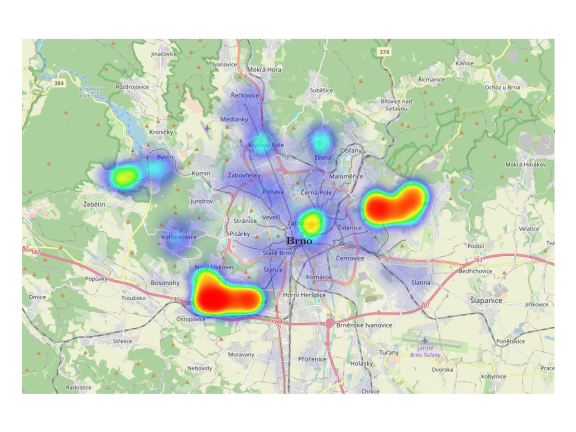
\includegraphics[width=1\textwidth]{obrazky-figures/ch2/select-locations-example.png}
	\caption{Example of selecting possible locations after the kernel density estimation. Here, the same estimated kernel density was used from figure \ref{fig:kernelDensityExample}.}
	\label{fig:selectPossibleLocations}
\end{figure}


\section{Multi-criteria Decision Analysis}

Areas with higher concentrations of potential clients were identified through the kernel density analysis, the next step involves evaluating and rating potential sites based on their geographic and physical characteristics. This rating process aims to prioritize locations that contain favourable attributes for establishing new commercial establishments---this is where multi-criteria decision analysis comes into play \cite{roig2013retail}.

Multi-Criteria Decision Analysis (MCDA) is a systematic approach employed in decision-making processes that involve the evaluation of multiple alternatives. This analytical method addresses the complexity of decision problems by considering various criteria simultaneously, providing a structured framework for assessing and comparing potential options~\cite{durbach2012modeling}.

In many decision-making scenarios, particularly those involving site selection, decision-makers are faced with multiple factors that influence the outcome, such as sales floor area, accessibility, potential market, and distance to competition \cite{roig2013retail}. 
These factors are often referred to as criteria.

In order to help the retailer evaluate multiple criteria, there is a variety of methods, such as PROMTHEE, ELECTRE, TOPSIS, AHP or Hybrid methodologies \cite{yap2019systematic}. According to \cite{roig2013retail}, the AHP method was selected.

\subsection{Analytic Hierarchy Process}
\label{subsec:ahp}

The Analytic Hierarchy Process (AHP) is considered to be the most popular among the others \cite{taherdoost2023comprehensive}. The method was proposed by Saaty as a pairwise comparison-based methodology \cite{saaty1988analytic}. 

\subsubsection{Hierarchical Structure of AHP}

\begin{figure}[ht]
	\centering
	\includesvg[width=1\textwidth]{obrazky-figures/ch2/hierarchical-model.svg}
	\caption{Hierarchical model (Adopted from \cite{roig2013retail})}
	\label{fig:ahp-structure}
\end{figure}

What all multi-criteria methods have in common is that most decisions can be improved by decomposing the overall evaluation of alternatives into evaluations on a number of criteria relevant to the problem \cite{durbach2012modeling}. The AHP method takes advantage of that by structuring decision problems into a comprehensive hierarchy which consists of several levels \cite{taherdoost2023comprehensive} (Figure \ref{fig:ahp-structure}).

The first level of the hierarchy is a goal of the process, sub-levels are constructed of criteria that can affect the choice. The last level of the hierarchy contains the alternatives, which are, at the end of the process, assessed.

\subsubsection{Application}

To illustrate this method, let's consider the following example. 

Suppose there are three projects: Project A, Project B and Project C. Using an analytical hierarchical process it is possible to identify the relative priority of each project. The goal is the project. Let's assume there are three criteria that drive the choice of project: duration, cost, and expected quality (In reality, there may be many more such criteria).

Let's use a 1-9 scale to compare criteria, define the significance of other attributes and put it into the table (Table \ref{tab:ahp-example-1}):

\begin{table}[ht]
\label{tab:ahp-example-1}
    \centering
    \begin{tabular}{|c|c|c|c|}
        \hline
         & Duration & Cost & Quality \\
        \hline
        Duration & 1 & 0.333 & 0.200 \\
        \hline
        Cost & 3 & 1 & 0.333 \\
        \hline
        Quality & 5 & 3 & 1 \\
        \hline
    \end{tabular}
    \caption{Criteria that are compared in pairs.}
\end{table}

Now let's calculate the sum of each column and divide the value of each cell by the sum of the values of the corresponding column (Table \ref{tab:ahp-example-2}).

\begin{table}[ht]
\label{tab:ahp-example-2}
    \centering
    \begin{tabular}{|c|c|c|c|}
        \hline
         & Duration & Cost & Quality \\
        \hline
        Duration & 0.111 & 0.077 & 0.130 \\
        \hline
        Cost & 0.333 & 0.231 & 0.217 \\
        \hline
        Quality & 0.556 & 0.692 & 0.652 \\
        \hline
    \end{tabular}
    \caption{Each value from previous table \ref{tab:ahp-example-1} divided by sum of each column.}
\end{table}

By calculating the average values of the rows, it is possible to find the specific weight of each of the criteria (\ref{tab:ahp-example-3}).

\begin{table}[ht]
\label{tab:ahp-example-3}
    \centering
    \begin{tabular}{|c|c|c|}
        \hline
        Duration & Cost & Quality \\
        \hline
        0.106 & 0.261 & 0.633 \\
        \hline
    \end{tabular}
    \caption{Weights of each of the criteria.}
\end{table}

Let's assume that each of the projects has the following attributes (Table \ref{tab:ahp-example-4}):

\begin{table}[ht]
\label{tab:ahp-example-4}
    \centering
    \begin{tabular}{|c|c|c|c|}
        \hline
         & Project A & Project B & Project C \\
        \hline
        Duration & 5 & 3 & 7 \\
        \hline
        Cost & 7 & 5 & 3 \\
        \hline
        Quality & 3 & 7 & 5 \\
        \hline
    \end{tabular}
    \caption{Project attributes.}
\end{table}

Taking each of the estimates with the specific weight of the criterion found earlier and adding them up in a project-by-project manner, we get:

$$\text{Project A} = 0.106 \cdot 5 + 0.261 \cdot 7 + 0.633 \cdot 3 = 4.256$$
$$\text{Project B} = 0.106 \cdot 7 + 0.261 \cdot 5 + 0.633 \dot 3 = 6.054$$
$$\text{Project C} = 0.106 \cdot 3 + 0.261 \cdot 7 + 0.633 \cdot 5 = 4.690$$


Obviously, \textbf{Project B} will be selected.

\subsubsection{Limitations}

 The user is able to define his judgements on a 1-9 scale, so rather than prescribing a ``correct`` decision, the AHP helps decision makers find the decision that best suits their goal and their understanding of the problem. The method faces the disadvantage of uncertainty and inconsistency in judgment and ranking criteria, which means the decision-maker may not know how to judge specific criteria, which leads to another flaw---it is possible for a rank reversal to occur \cite{taherdoost2023comprehensive}. In order to detect this flaw, it is possible to calculate consistency, which is estimated using the consistency ratio, which reflects how consistent the judgements are relative to large samples of purely random judgments. If the consistency ratio exceeds 10\%, the judgments are considered untrustworthy \cite{saaty1992decision}.

\subsubsection{Important Criteria for Site Selection Process}

According to \cite{roig2013retail}, there are four main criteria: establishment, location, demographic factors and competition (Figure \ref{fig:ahp-criteria}):

\begin{figure}[ht]
	\centering
	\includesvg[width=1\textwidth]{obrazky-figures/ch2/ahp-criteria.svg}
	\caption{Factors that affect the success of a supermarket (Adopted from \cite{roig2013retail})}
	\label{fig:ahp-criteria}
\end{figure}

\begin{enumerate}
    \item \textbf{Establishment}---refers to the features of the property itself. These features encompass the size of the sales floor area, whether there is parking, the number of product departments, and the available number of checkouts \cite{roig2013retail}.
    \item \textbf{Location}---covers all aspects related to where the store is situated. This includes how easy it is to reach by car or on foot, its visibility to potential clients, and the amount of passing trade in the surrounding area \cite{roig2013retail}.
    \item \textbf{Demographics}---is about understanding the characteristics of the people living in the trade area of the new retail site. This involves considering the total population in the trade area, the specific types of clients based on factors like purchasing power and family structure, predictions for growth in the surrounding area, and variations in sales throughout the year \cite{roig2013retail}.
    \item \textbf{Competition}---focuses on the features of other establishments that offer similar services. This takes into account the distance to competitors, how well-known their brand is in the area, the size of their sales floor area, and the type of commercial strategy they employ \cite{roig2013retail}.
\end{enumerate}

The decision-making process involved a diverse group of retail site location and marketing experts, individuals from both academic and professional backgrounds. Each expert participated in interviews where they assessed and rated various criteria crucial for retail site selection (Figure \ref{fig:ahp-criteria}). The comparison matrix derived from these evaluations served as a foundation for determining the significance of each criterion. During the analysis, scores with a consistency ratio exceeding 10\% were excluded to maintain the reliability of the results \cite{roig2013retail}.

The next step involved extracting eigenvectors associated with each matrix, representing the expert's individual judgments. These eigenvectors were then aggregated using the arithmetic mean technique, resulting in a set of weights associated with each criterion. These weights, reflecting the experts' consensus on the importance of each criterion, were subsequently used to rank the sub-criteria \cite{roig2013retail}.

\begin{table}[ht]
\centering
\begin{tabular}{|c|p{3cm}|p{5cm}|r|}
\hline
\textbf{Ranking} & \textbf{Criteria} & \textbf{Subcriteria} & \textbf{Score} \\
\hline
1 & Location (0.509) & Volume of passing trade (0.342) & 17.44\% \\
2 & Location (0.509) & Visibility (0.287) & 14.62\% \\
3 & Competition (0.245) & Distance to competition (0.591) & 14.49\% \\
4 & Demographics (0.188) & Potential market (TA) (0.519) & 9.75\% \\
5 & Location (0.509) & Accessibility by car (0.191) & 9.71\% \\
6 & Location (0.509) & Accessibility by foot (0.180) & 9.17\% \\
7 & Competition (0.245) & Brand recognition (0.227) & 5.56\% \\
8 & Demographics (0.188) & Seasonality (0.250) & 4.69\% \\
9 & Establishment (0.057) & Number of departments (0.575) & 3.30\% \\
10 & Competition (0.245) & Type of competition (0.128) & 3.13\% \\
11 & Demographics (0.188) & Growth in the area (0.147) & 2.75\% \\
12 & Demographics (0.188) & Socio-demographic characteristics (0.085) & 1.60\% \\
13 & Competition (0.245) & Size of competition (0.055) & 1.35\% \\
14 & Establishment (0.057) & Sales floor area (0.179) & 1.03\% \\
15 & Establishment (0.057) & Parking (0.154) & 0.88\% \\
16 & Establishment (0.057) & Number of checkouts (0.092) & 0.53\% \\
\hline
\end{tabular}
\caption{Ranking of the subcriteria that determine the success of a supermarket (Adopted from \cite{roig2013retail})}
\label{tab:expert-rating}
\end{table}

According to the insights (Table \ref{tab:expert-rating}) gathered from the consulted experts, the critical factors influencing a supermarket's success are primarily the volume of passing trade (17.44\%), store visibility (14.62\%), proximity to competitors (14.49\%), the potential market within the trade area (9.75\%), accessibility by car (9.71\%), and accessibility by foot (9.17\%). The collective impact of these six sub-criteria accounts for more than 75\% of a supermarket's success.

